\documentclass[12pt]{article}
\usepackage{iftex}
\usepackage{graphicx}
\usepackage{enumitem}
\usepackage{hyperref}
\usepackage[style=apa, backend=biber]{biblatex}
\addbibresource{phd_bombus.bib}
\setcounter{maxnames}{20}
\setcounter{minnames}{1}
\usepackage{color}
\usepackage{amsmath}
\usepackage{amssymb}
\usepackage[export]{adjustbox}
\usepackage{verbatim}
\usepackage{mathpazo}
\usepackage{setspace}
\usepackage{multirow}
\usepackage{lscape}
\usepackage{fancyhdr}
\usepackage[normalem]{ulem}
\usepackage{rotating}
\usepackage{chngcntr}
\usepackage{float}
\usepackage[parfill]{parskip}
\usepackage[tiny,compact]{titlesec}
\usepackage{longtable}
\usepackage{textcomp}
\usepackage{rotating}
\usepackage{xr}
\usepackage{caption}
\usepackage{siunitx}
\usepackage[T1]{fontenc}
\usepackage{gensymb}
\sisetup{round-mode=places, round-precision=2, detect-all}

\newcommand{\flagged}[1] {
  \textcolor{blue}{#1}
}

\hypersetup{colorlinks=true, linkcolor=black, citecolor=black}
\RequirePackage{lineno}

\renewcommand{\thefigure}{A\arabic{figure}}  % Prefix figures with "A"
\setcounter{figure}{0}  % Reset figure counter
\renewcommand{\thetable}{A\arabic{table}}
\setcounter{table}{0}
\setcounter{section}{0}

\def\title{Appendix 1 -- Population Genetics and Colony Assignments}



\begin{document}
\begin{center}
  {\large \title \par}
\end{center}\par

\section{Assessing locus $F_{is}$, $F_{st}$ and linkage disequilibrium}

\begin{figure}[H]
    \centering
    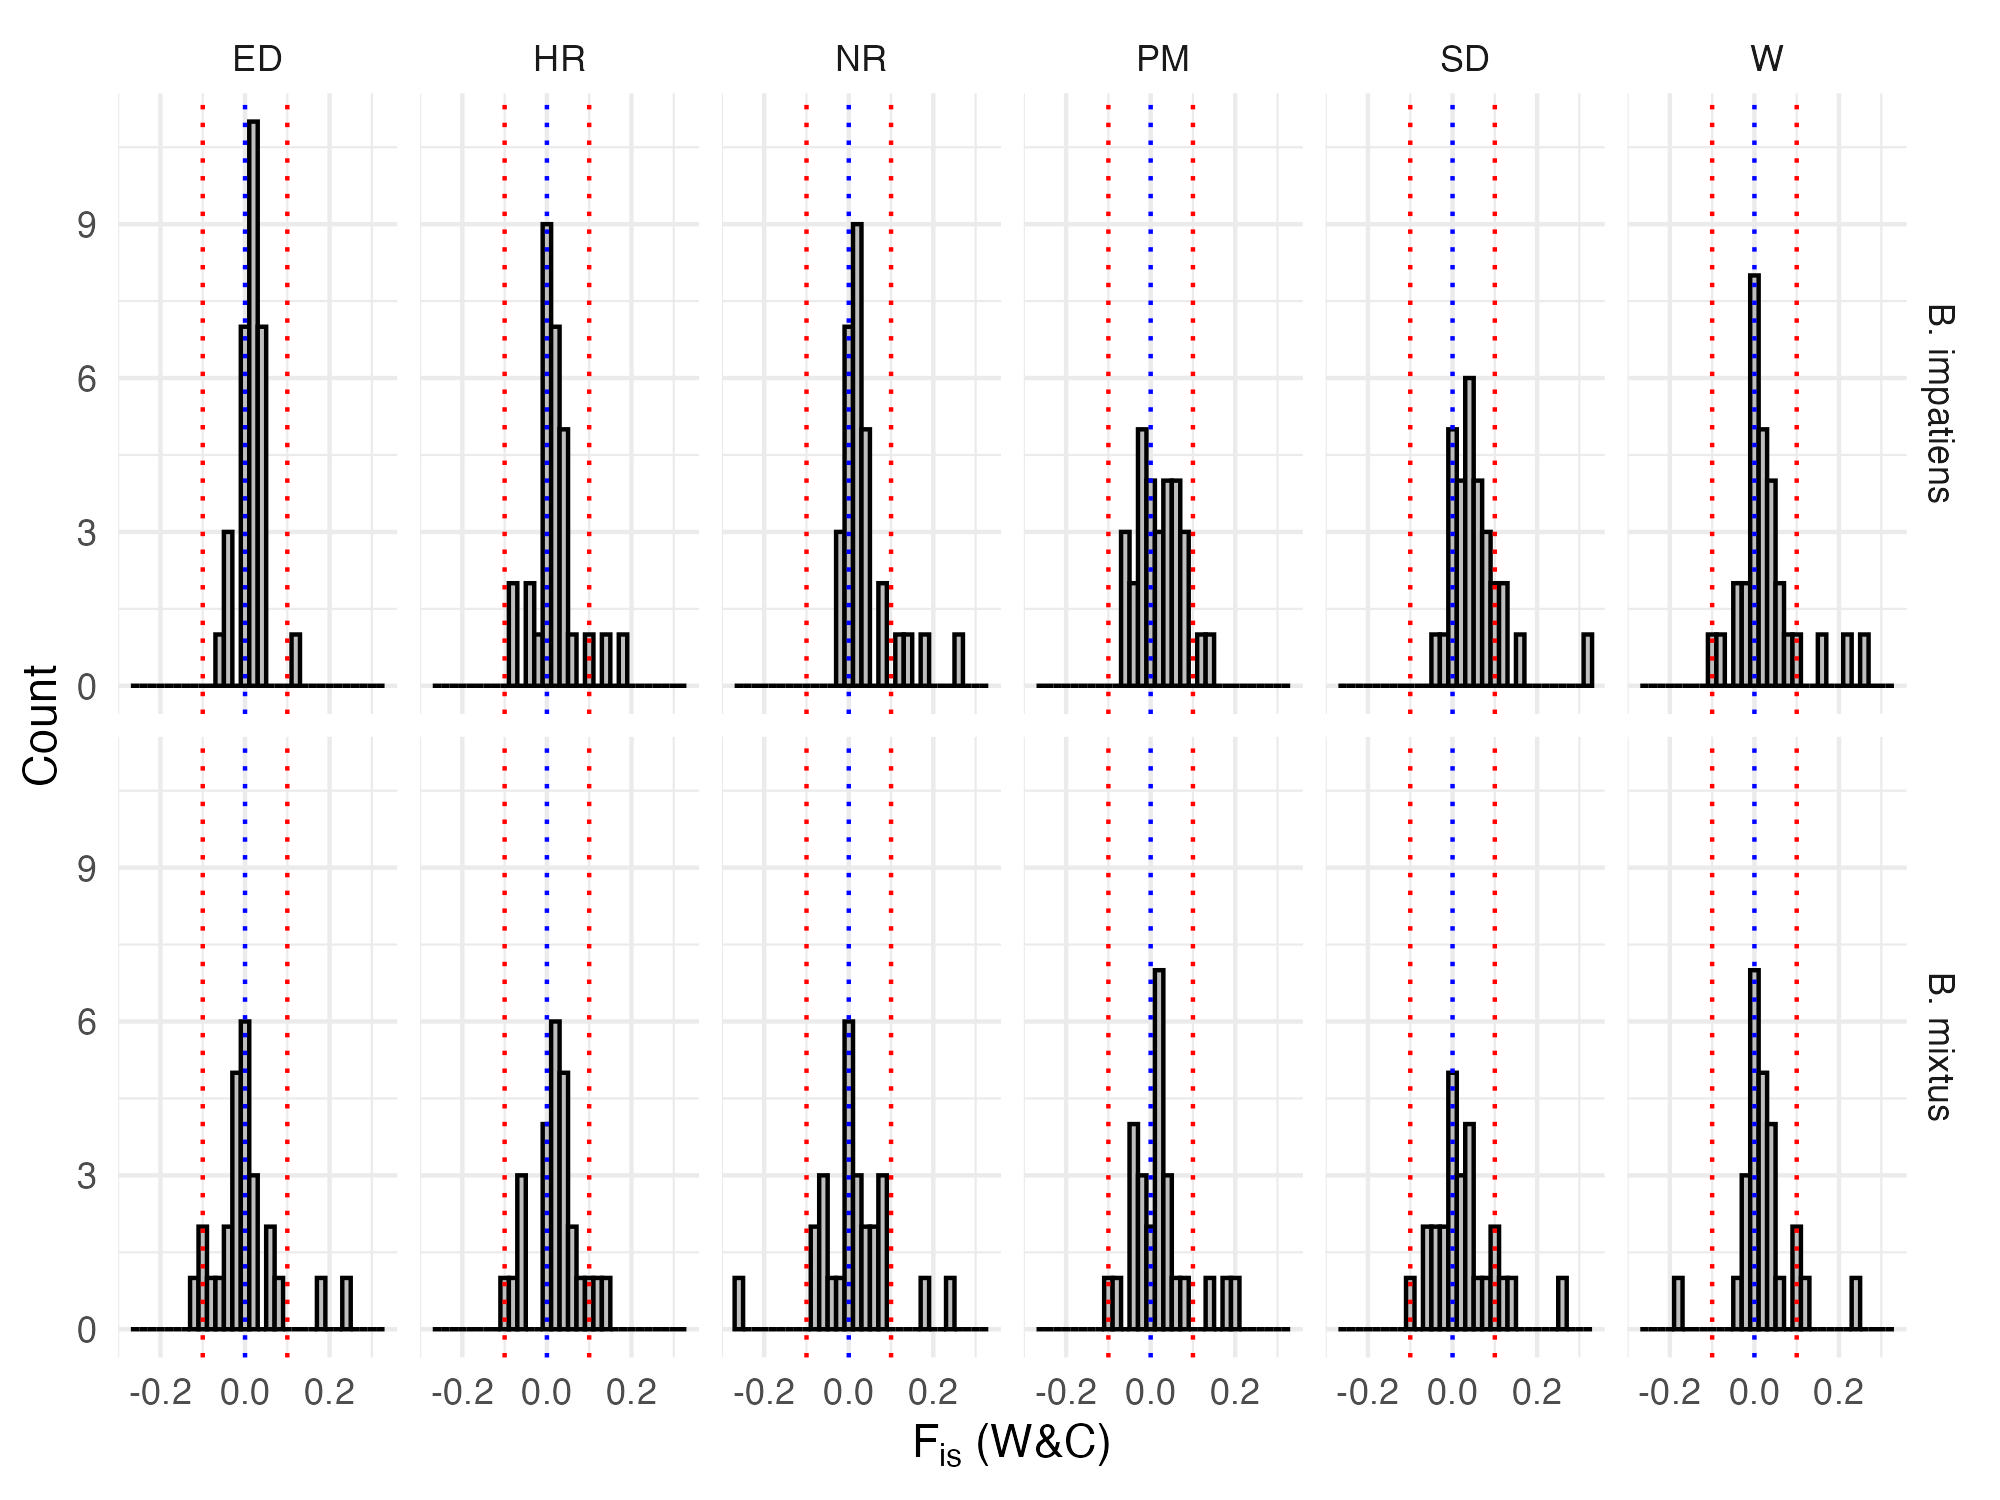
\includegraphics[width=\linewidth]{appendix_figures/Fis.jpg}
    \caption{Estimates of $F_{is}$ for each locus in each subpopulation. Estimates from 2022 and 2023 were calculated separately but are shown together for each site x species combination. Blue dotted lines indicates $F_{is} = 0$ and red dotted lines indicate $F_{is} = \pm 0.1$.}
    \label{fig:Fis}
\end{figure}


\begin{figure}[H]
    \centering
    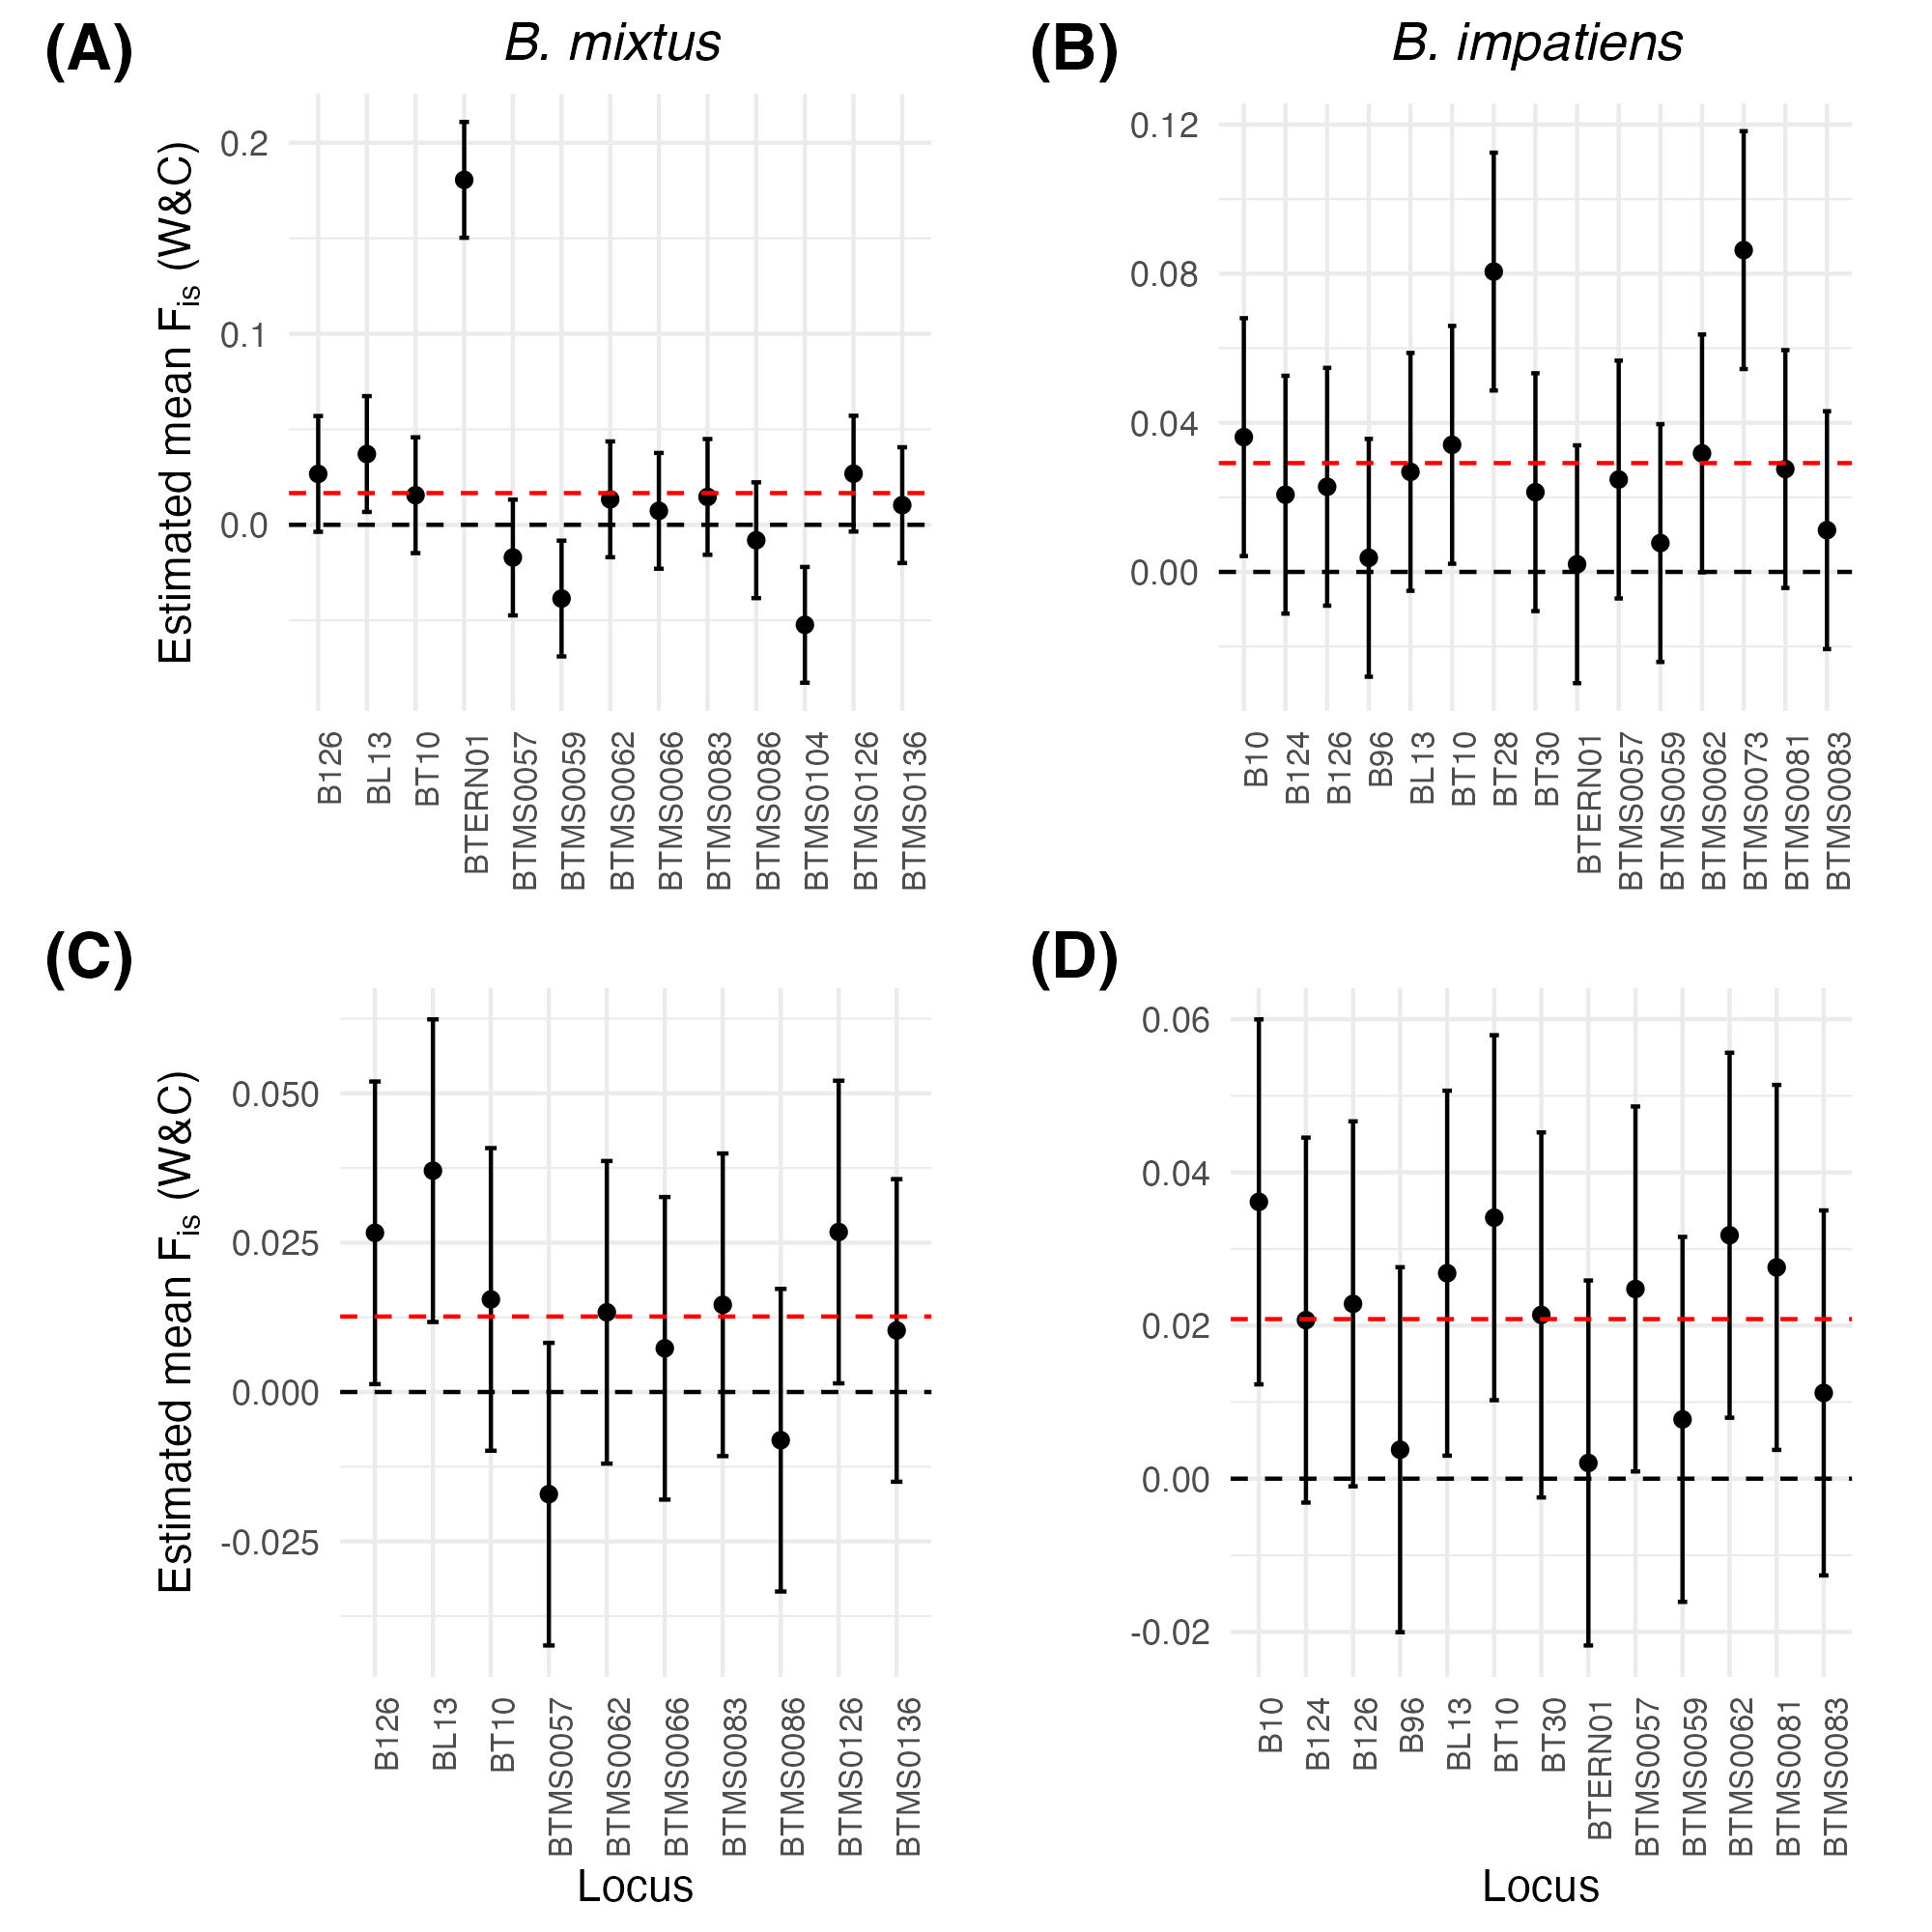
\includegraphics[width=\linewidth]{appendix_figures/marginalmeans.jpg}
    \caption{Locus-specific $F_{is}$ marginal means. A) \emph{B. mixtus} all loci; B) \emph{B. impatiens} all loci; C) \emph{B. mixtus} loci following iterative removal of loci which differed significantly from global mean $F_{is}$; D) \emph{B. impatiens} loci following iterative removal of loci which differed significantly from global mean $F_{is}$. Dashed black line denotes $F_{is} = 0$, dashed red line denotes global mean $F_{is}$ for each species.}
    \label{fig:marginalmeans}
\end{figure}


\begin{figure}[H]
    \centering
    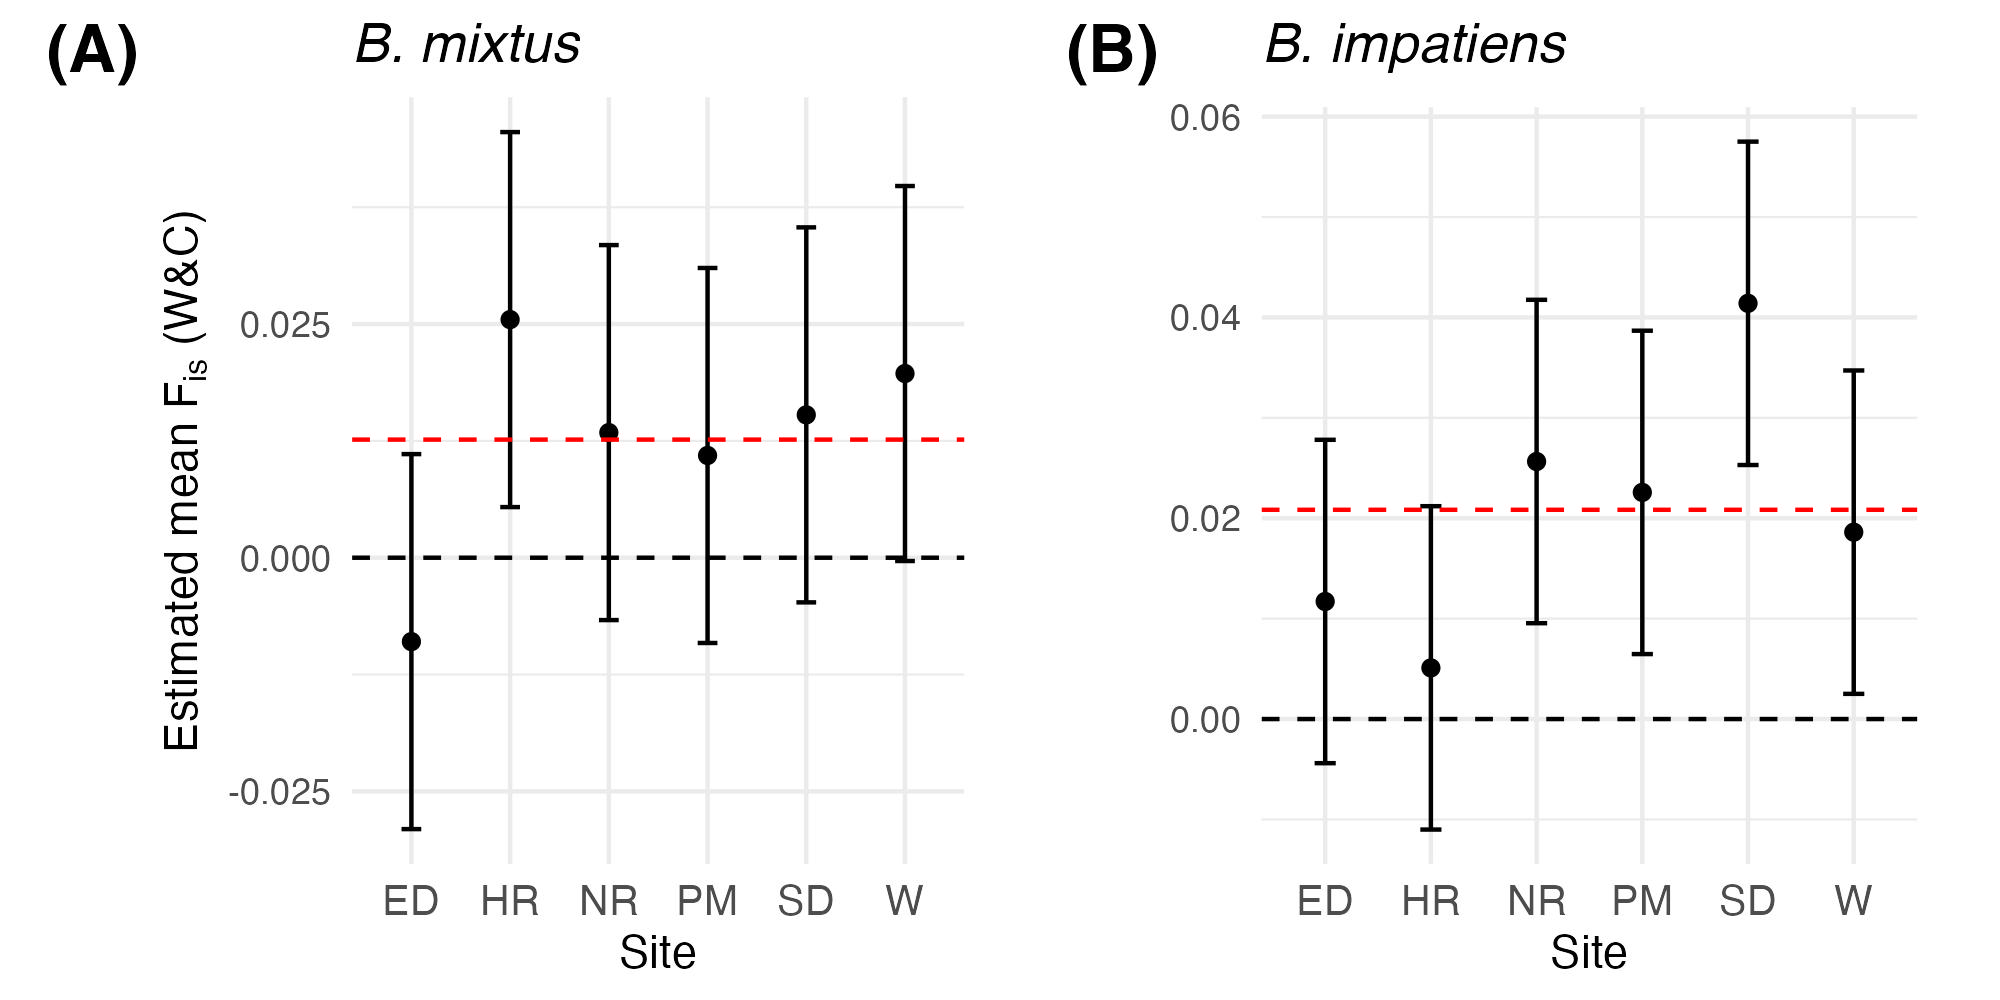
\includegraphics[width=\linewidth]{appendix_figures/siteFis.jpg}
    \caption{Site-specific $F_{is}$ marginal means following removal of low-quality loci for A) \emph{B. mixtus} and B) \emph{B. impatiens}. Dashed black line denotes $F_{is} = 0$, dashed red line denotes global mean $F_{is}$ for each species.}
    \label{fig:siteFis}
\end{figure}


\section{Testing COLONY on simulated data}
To test the informativeness of our genetic loci and validate the accuracy of COLONY version 2.0.6.5 \parencite{jonesCOLONYProgramParentage2010} for accurately detecting siblingships amongst our specimens, we performed simulations using realistic family sizes, spatial distributions, and allelic frequencies present in our true data.

We approached these simulations with four objectives:

(i) To determine false positive and false negative siblingship assignment rates, given the informativeness of our microsatellite datasets, 

(ii) To inform an appropriate strategy (probability threshold, number of runs of the software) for maintaining or rejecting each sibling pair;

(iii) To select suitable software parameters, and in particular to evaluate the usefulness of siblingship size priors and exclusion of between-site siblingships for reducing false positive rates;

(iv) To assess whether modelling female polygamy would improve family reconstruction in cases for which sibling genotypes were simulated under varying rates of multiple paternity.

\subsection{Simulation strategy}

\subsubsection{Spatially explicit siblingships}
We first simulated spatially explicit siblingships following \textcite{popeInferringForagingRanges2017}. We began by simulating six 5 x 5 trapping grids (e.g., 25 traps total at locations $k \in \kappa$) on a single raster surface comprised of cells $j \in \mathbb{J}$. Colonies $i \in \mathbb{C}$ were distributed uniformly at random throughout the ``landscape" (Fig. \ref{fig:simulations} A-B).

We then sampled individuals from colonies $i \in \mathbb{C}$ captured at traps $k \in \mathbb{K}$ from the joint distribution $\Pr(s, c \mid s \in \kappa)$, where $\{s,c\}$ are the indices of a random visitation event of an individual from colony $c \in \mathbb{C}$ to grid cell $s \in \mathbb{J}$.

To do this, we first sampled a trap ($k$) from

\[
\Pr(s = k \mid s \in \kappa) \;=\; \frac{\Pr(s = k)}{\Pr(s \in \kappa)} \tag{1}
\]

where

\[
\Pr(s = k) \;=\; \sum_{i \in C} \Pr(s = k \mid c = i)\,\Pr(c = i)
\]

and

\begin{align*}
\Pr(s \in \kappa) 
    &= \sum_{i \in \mathbb{C}} \Pr(s \in \kappa \mid c = i)\,\Pr(c = i) \\[0.5em]
    &= \sum_{i \in \mathbb{C}} \sum_{k \in \kappa} \Pr(s = k \mid c = i)\,\Pr(c = i)
\end{align*}


Combining these statements gives a probability of sampling from trap $k$ of:

\[
\Pr(s = k \mid s \in \kappa) \;=\; \frac{\sum_{i \in C} \Pr(s = k \mid c = i)\,\Pr(c = i)}{\sum_{i \in \mathbb{C}} \sum_{k \in \kappa} \Pr(s = k \mid c = i)\,\Pr(c = i)} \tag{2}
\]

We then sampled a colony ($i$) from

\begin{align*}
\Pr(c = i \mid s = k)
  &= \frac{\Pr(s = k \mid c = i) \Pr(c = i)}{\Pr(s = k)} \\[0.5em]
  &= \frac{\Pr(s = k \mid c = i) \Pr(c = i)}{\sum_{i \in \mathbb{C}} \Pr(s = k \mid c = i)\,\Pr(c = i)} \tag{3}
\end{align*}


We define the foraging kernel of workers from colony $i$ as

\[
\Pr(s = k \mid c = i)
\;=\; 
\frac{\lambda_i(k)}{\sum_{j \in J} \lambda_i(j)} \tag{4}
\]

where the visitation intensity of individuals from colony $i$ to location $j$ is 

\[
ln(\lambda_i(j)) = \frac{- \lVert x_j - \delta_i \rVert}{\rho} \tag{5}
\]

$x_j$ are the spatial coordinates of any grid cell in the raster, and $\delta_i$ are the spatial coordinates of colony $i$. The foraging kernel in this example is therefore assumed to be symmetrical and exponentially decaying as a function of distance from the colony location. This means that the total visitation of each colony across the landscape ($\sum_{j \in J} \lambda_i(j)$) is the same for all colonies, and can be represented using the constant $\mathbb{D}$. $\Pr(c = i)$ is the proportion of all bees in the landscape originating from colony $i$, e.g., $\Pr(c = i) = \frac{n_i}{N}$ where $n_i$ is the number of bees from colony $i$, and $N = \sum_{i \in \mathbb{C}} n_i$ is the total number of bees in the landscape.

Combining (4) with (2) and (3) gives the probability of sampling an individual from trap $k$

% with variable foraging kernels
%\[
%\Pr(s = k \mid s \in \kappa) \;=\; \frac{\sum_{i \in \mathbb{C}} \frac{\lambda_i(k)}{\sum_{j \in %J} \lambda_i(j)}\,\frac{n_i}{N}}{\sum_{k \in \kappa} \sum_{i \in \mathbb{C}} \frac{\lambda_i(k%)}{\sum_{j \in J} \lambda_i(j)}\,\frac{n_i}{N}}
%\]

% with identical foraging kernels
\[
\Pr(s = k \mid s \in \kappa) \;=\; \frac{\sum_{i \in \mathbb{C}} \lambda_i(k) \frac{n_i}{N}}{\sum_{k \in \kappa} \sum_{i \in \mathbb{C}} \lambda_i(k) \frac{n_i}{N}}
\]

and the probability that the individual originates from colony $i$

% with variable foraging kernels
% \[
% \Pr(c = i \mid s = k) \;=\;  \frac{\frac{\lambda_i(k)}{\sum_{j \in J} \lambda_i(j)} \frac{n_i}{N}}{\sum_{i \in \mathbb{C}} \frac{\lambda_i(k)}{\sum_{j \in J} \lambda_i(j)} \frac{n_i}{N}}
% \]

% with identical foraging kernels
\[
\Pr(c = i \mid s = k) \;=\; \frac{\lambda_i(k) \frac{n_i}{N}}{\sum_{i \in \mathbb{C}} \lambda_i(k) \frac{n_i}{N}}
\]

For each simulation, samples are drawn from $\Pr(s, c \mid s \in \kappa)$ until a stopping point (desired number of samples) is reached. $n_i$ is updated after each ``sampling event" to prevent oversampling from colonies located very close to traps.

To verify that the size of sampled siblingships (e.g., number of siblings per sibling group) accurately mirrors the distribution of siblingship sizes in real data, we compared our simulated distributions to the distribution of siblingshp sizes in our real data (Fig. \ref{fig:simulations} C-D). For this simulation strategy, we found that moderating the background density of colonies (i.e., the total number of colonies simulated on the landscape) was the most effective strategy for controlling average siblingship size. A larger number of simulated colonies resulted in a higher proportion of singleton colonies (colonies represented by only a single individual).

\begin{figure}[H]
    \centering
    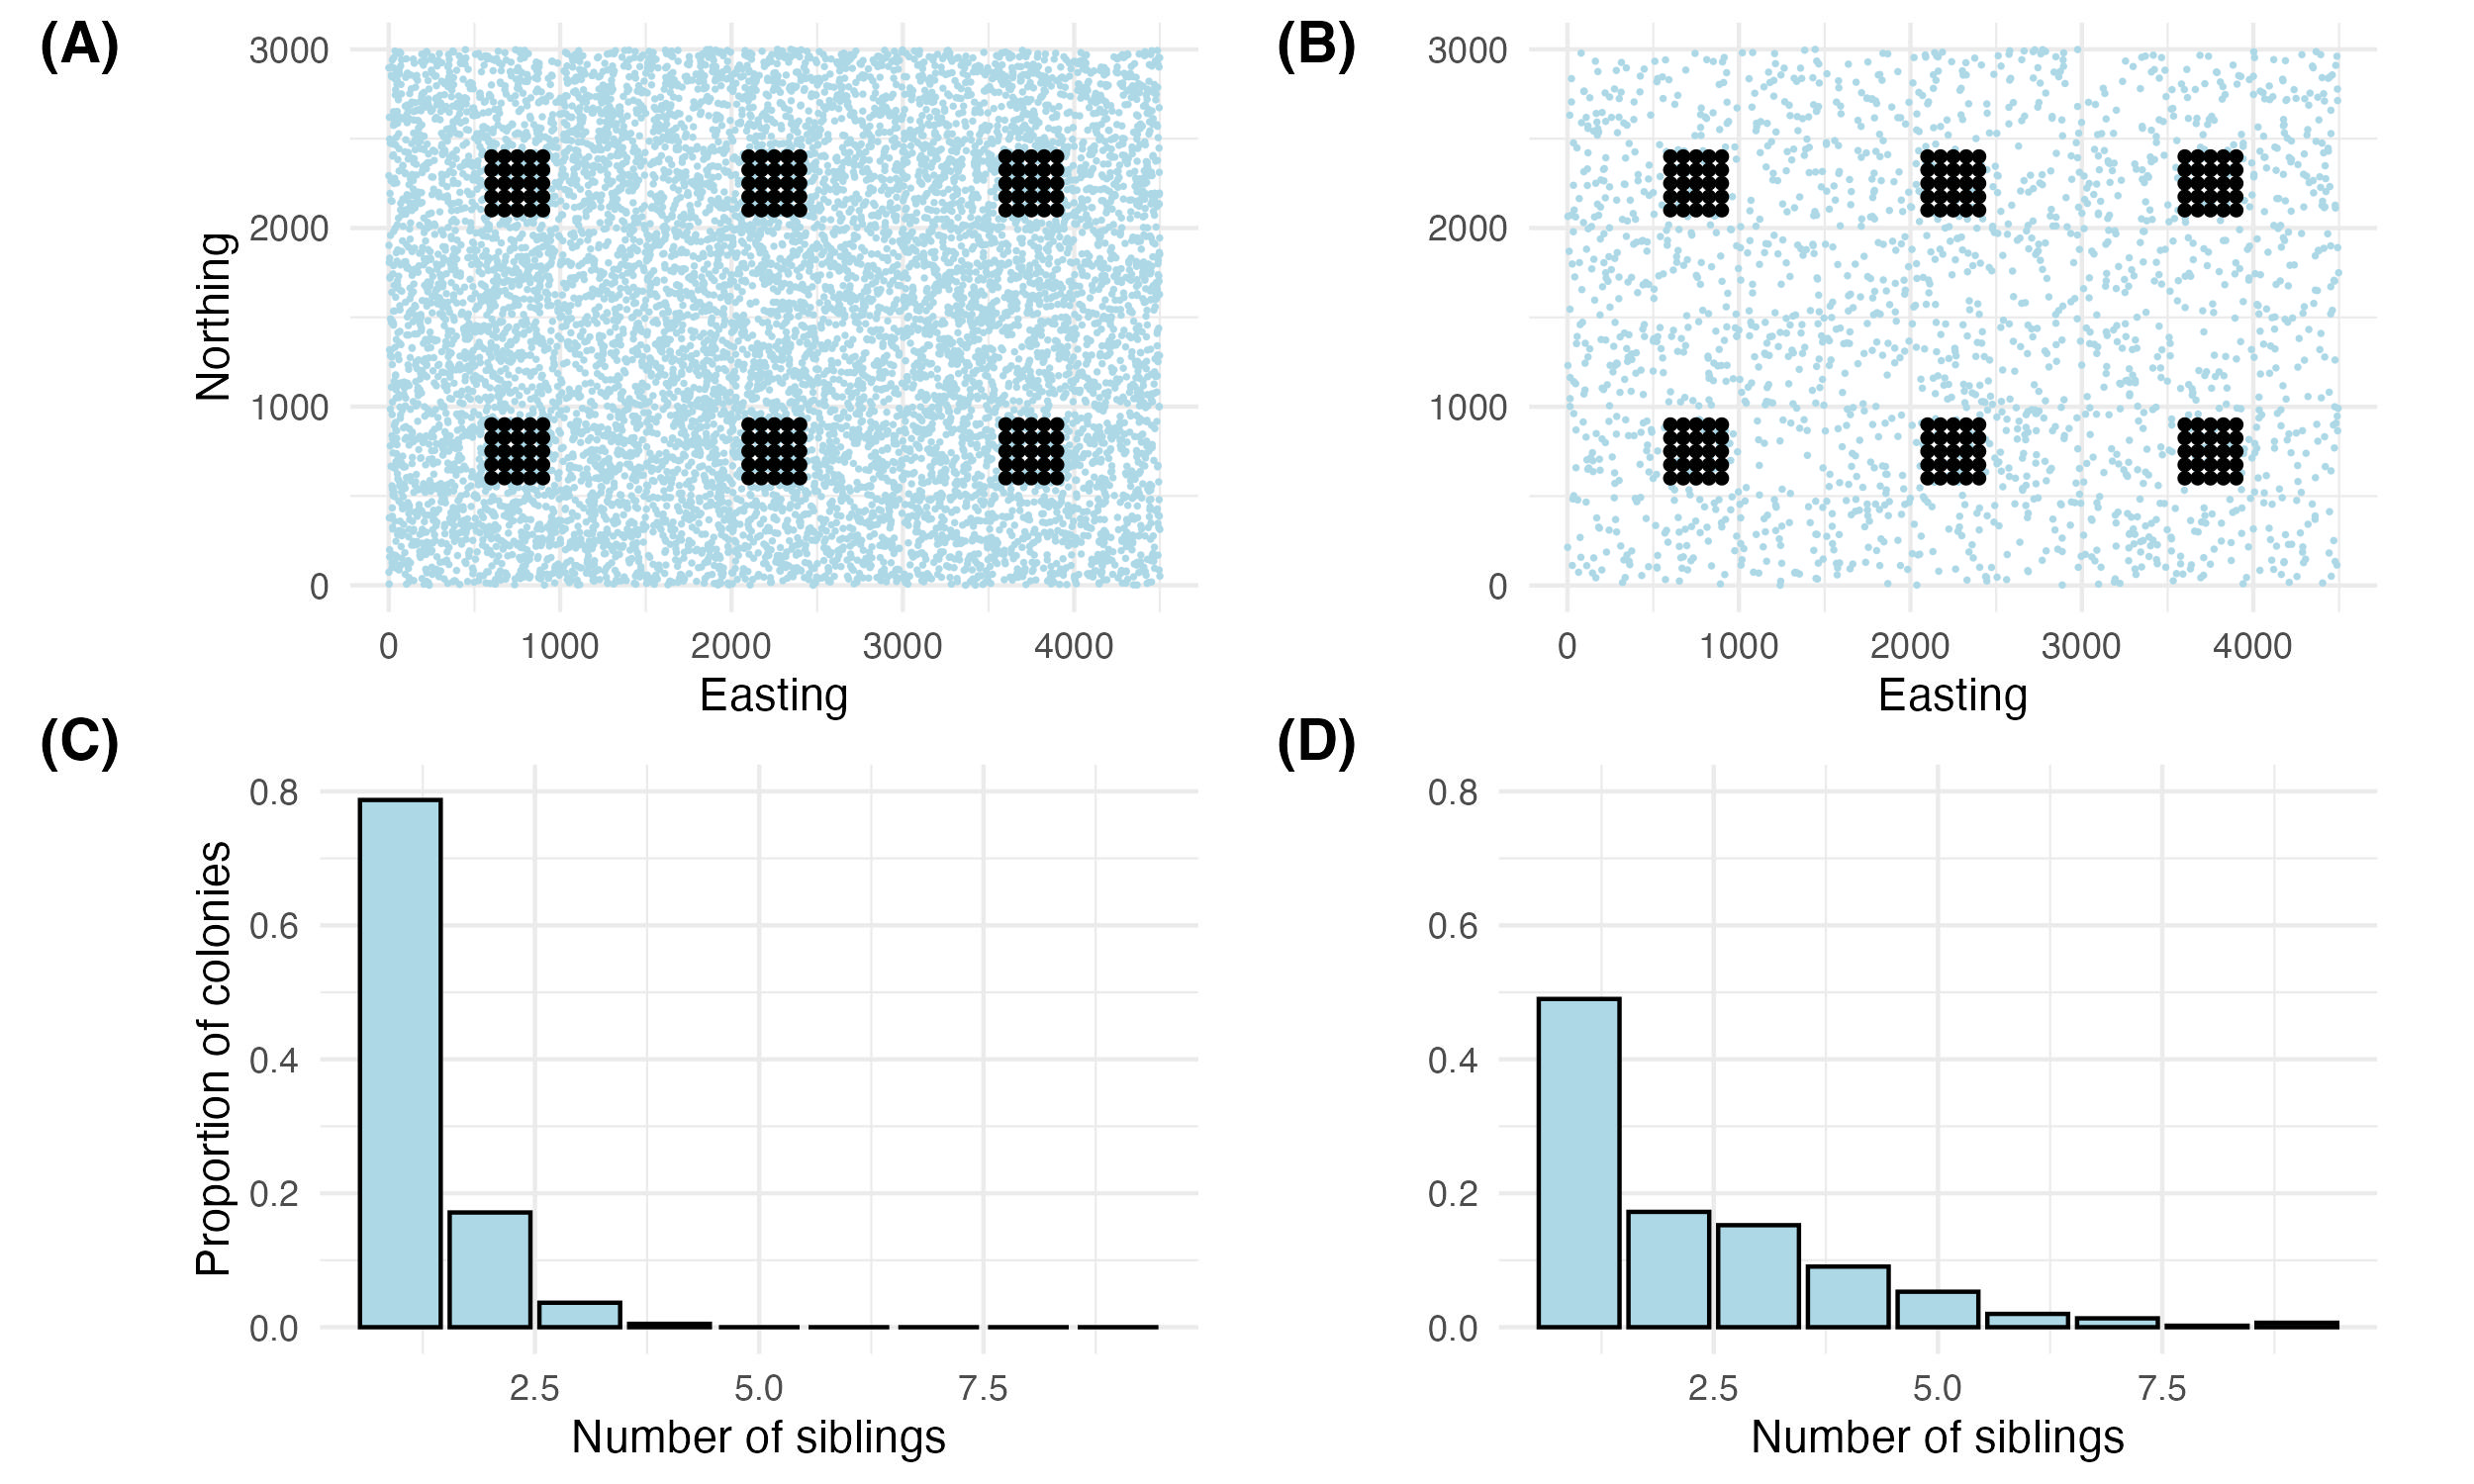
\includegraphics[width=\linewidth]{appendix_figures/simulations.jpg}
    \caption{Simulations of spatially explicit siblingships. (A-B) Spatial distribution of traps (black points) and simulated colonies (light blue points). (C-D) Distribution of siblingship sizes in final simulated datasets. (A,C) Simulations using 10,000 background colonies. (B,D) Simulations using 2,000 background colonies. In general, a higher background density of colonies results in a smaller average family size; in both cases, some colonies are not observed in the final dataset. Each map unit in our simulation represents 5 meters (e.g., 1000 map units = 5000 meters). The background colony densities represented here therefore equate to 0.26 colonies per hectare and 0.06 colonies per hectare; we use the former value, as it is in line with previous estimates of landscape-wide colony densities and creates a more realistic distribution of siblingship sizes (C).}
    \label{fig:simulations}
\end{figure}


\subsubsection{Multilocus genotypes}
We simulated multilocus genotypes for each sampled individual under several mating scenarios. In the simplest case, we assume monogamy for both males and queens. The majority of the simulation results presented below follow this assumption. In a second set of simulations, we assumed varying rates of polyandry (e.g., queen polygamy) to assess the impact of this paradigm on siblingship inference. For each simulation we used the following heuristic:

(i) Simulate parental genotypes for each siblingship based on the allele frequencies present in our real data. These frequencies were inferred from an earlier run of COLONY, which provides estimated frequencies after accounting for heightened frequency of alleles present in large families; because average family size was small in our dataset (< 2 individuals) and large families were rare (Fig \ref{fig:simulations} C), raw allele frequencies would have likely been sufficient.

(ii) Randomly draw offspring genotypes from the set of possible parental alleles at each locus. For simulations involving monogamous mating, father haplotypes are assigned directly to all offspring in the siblingship; in colonies with multiple paternity, we assume two fathers and assign inheritance of paternal haplotypes from $\Pr(father_1, father_2) = (0.7, 0.3)$ following the proportions observed for \emph{B. impatiens} in \textcite{birdMatingFrequencyEstimation2024}.

(iv) Introduce errors and data missingness based on observed rates for our real datasets. To introduce errors, we mutate each allele with a probability equal to the rate of errors for that locus and species; we assume that most errors are due to contamination, rather than allele dropout, and therefore draw new (erroneous) alleles from the allele frequency distribution for each species. We observed that individuals which were missing data for \emph{one} copy of a locus were more likely to be missing data for \emph{both} copies than if missingness were distributed uniformly at random. This is likely because there were two primary missingness-generating processes in real data: amplification failure (both alleles missing for an individual) and binning failure (one or both alleles missing for an individual). (In cases where only one copy of a locus failed to amplify, heterozygous individuals would be falsely classified as homozygous---an error, rather than missing data). To mimic the observed distribution of missingness, we first calculate the proportion of missing data for each marker ($P_{missing}$) and then remove data for (1) both alleles, with probability $1/3 * P_{missing}$ and for (2) a single allele, with probability $1/3 * P_{missing}$.

This method allows us to draw conclusions based on the informativeness of our specific genetic datasets, rather than based on an idealized situation with perfect data. We performed simulations based on allele frequencies for both species (\emph{B. mixtus} and \emph{B. impatiens}) because variation in marker number and/or polymorphic information content could lead to differing results.

\subsection{Determining an appropriate heuristic for maintaining or rejecting inferred siblingships}

Like any software for family reconstruction, COLONY can produce erroneous siblingships (false positives) or fail to identify kinship when it exists (false negatives). Our preliminary data analyses resulted in a high number of inferred siblingships between individuals separated by >20 km when individuals from all study sites were permitted to form siblingships. While the biology of bumblebee foraging/dispersal does not unilaterally exclude the possibility of such distant relationships, the likelihood of observing such separation distances is extremely small, and unlikely to represent biological reality except in very rare cases.

A common strategy in studies performing \emph{Bombus} colony assignment is to repeat multiple "runs" (usually 2-5) of the COLONY software on the dataset, and maintain family groups which are inferred in all runs at or above some confidence threshhold (usually $P \ge 0.95$, but sometimes $P \ge 0.8$). See, for example, \textcite{carvellMolecularSpatialAnalyses2012, raoBumbleBeeHymenoptera2012, dreierFinescaleSpatialGenetic2014a, geibBumbleBeeNest2015a, carvellBumblebeeFamilyLineage2017a, molaWildfireRevealsTransient2020a}. However, we are not aware of any studies which give support for a particular threshhold probability or number of runs necessary to reach a particular confidence level in assignments, nor to achieve a satisfactory balance between false positive siblingships and false negative siblingships. Indeed, the desirable threshhold is likely to vary as a function of the number and informativeness of markers for a given population.

To overcome these limitations, we tested probability exclusion criteria from $P = 0.95$ to $P = 1$, for 1 or 5 runs of COLONY version 2.0.6.5. Further, we compared the use of family cluster probabilities (COLONY output file .BestCluster---hereafter referred to as the family method) and full sibling dyad probabilities (COLONY output .FullSibDyad---hereafter referred to as the dyad method).

We began by simulating 5 datasets (e.g., different siblingship arrangements with unique parental genotypes) consisting of n = 1200 individuals each, which was roughly the midpoint of population sizes for our real data. For each dataset we performed 5 runs of COLONY (see Table \ref{tab:softwarespecs} for a summary of COLONY software settings).

Based on our results, we conclude that the software converges reliably for datasets like ours, and that repeated runs of the software have litte or no effect on conclusions drawn. In most cases, false positive and false negative rates are either identical or nearly overlapping, regardless of the numbers of runs (Fig \ref{fig:fpr_repetition}, \ref{fig:fnr_repetition}). We therefore recommend that to save time and computational resources, researchers should check for convergence for each microsatellite dataset using 2-3 runs of the software, and if convergence is achieved they should feel confident that a single run is sufficient to identify siblingships.

For both species we found that increasing the probability threshhold from 0.95 to 1 more effectively reduced false positives for the dyad method than for the family method; in general, a probability threshold $\ge$ 0.99 was necessary to maintain false positive rates at around 5\% using the dyad method. For $P = 1$ the dyad method led to a higher proportion of false negatives ($\ge 5\%$) (Fig \ref{fig:fnr_repetition}). For this reason, we would not recommend this stringent a threshold unless a very low rate of false positives is required.

\begin{figure}[H]
    \centering
    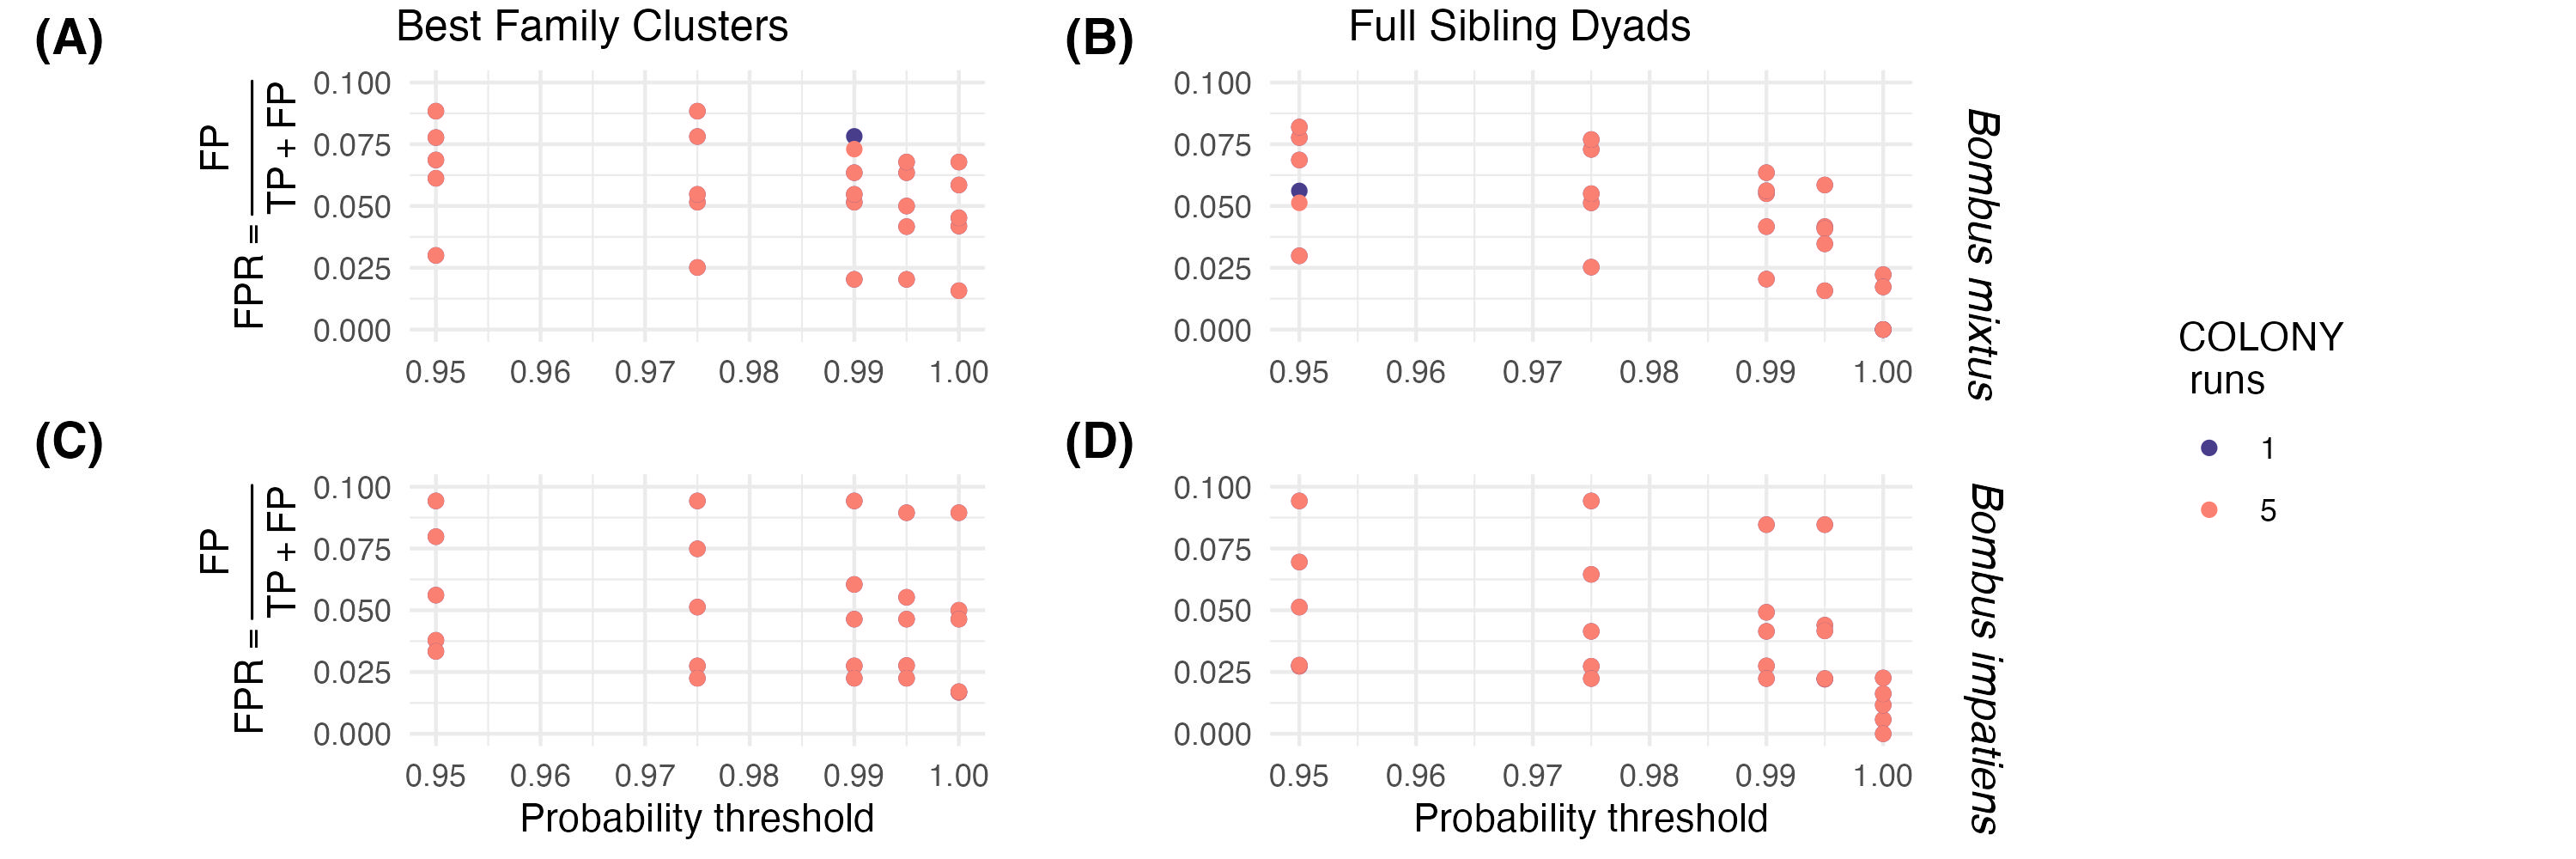
\includegraphics[width=\linewidth]{appendix_figures/fpr_repetition.jpg}
    \caption{False positive rates produced by COLONY 2.0.6.5 when assigning siblingships to simulated data based on \emph{B. mixtus} (A-B) and \emph{B. impatiens} (C-D) allele frequencies and marker numbers. Shown here as a function of the probability threshold used to maintain siblingships. (A, C): False positive rates when siblingships are assigned via the ``family" method (using .BestCluster output), (B, D): False positive rates when siblingships are assigned via the ``dyad" method (using .FullSibDyad output). Color denotes the number of replicated runs of the software used to establish siblingships; a high degree of overlap between the two methods (1 vs 5 runs) suggests that the results of each run are highly stable and that a single run is just as effective as five runs for excluding erroneous siblingships.}
    \label{fig:fpr_repetition}
\end{figure}

\begin{figure}[H]
    \centering
    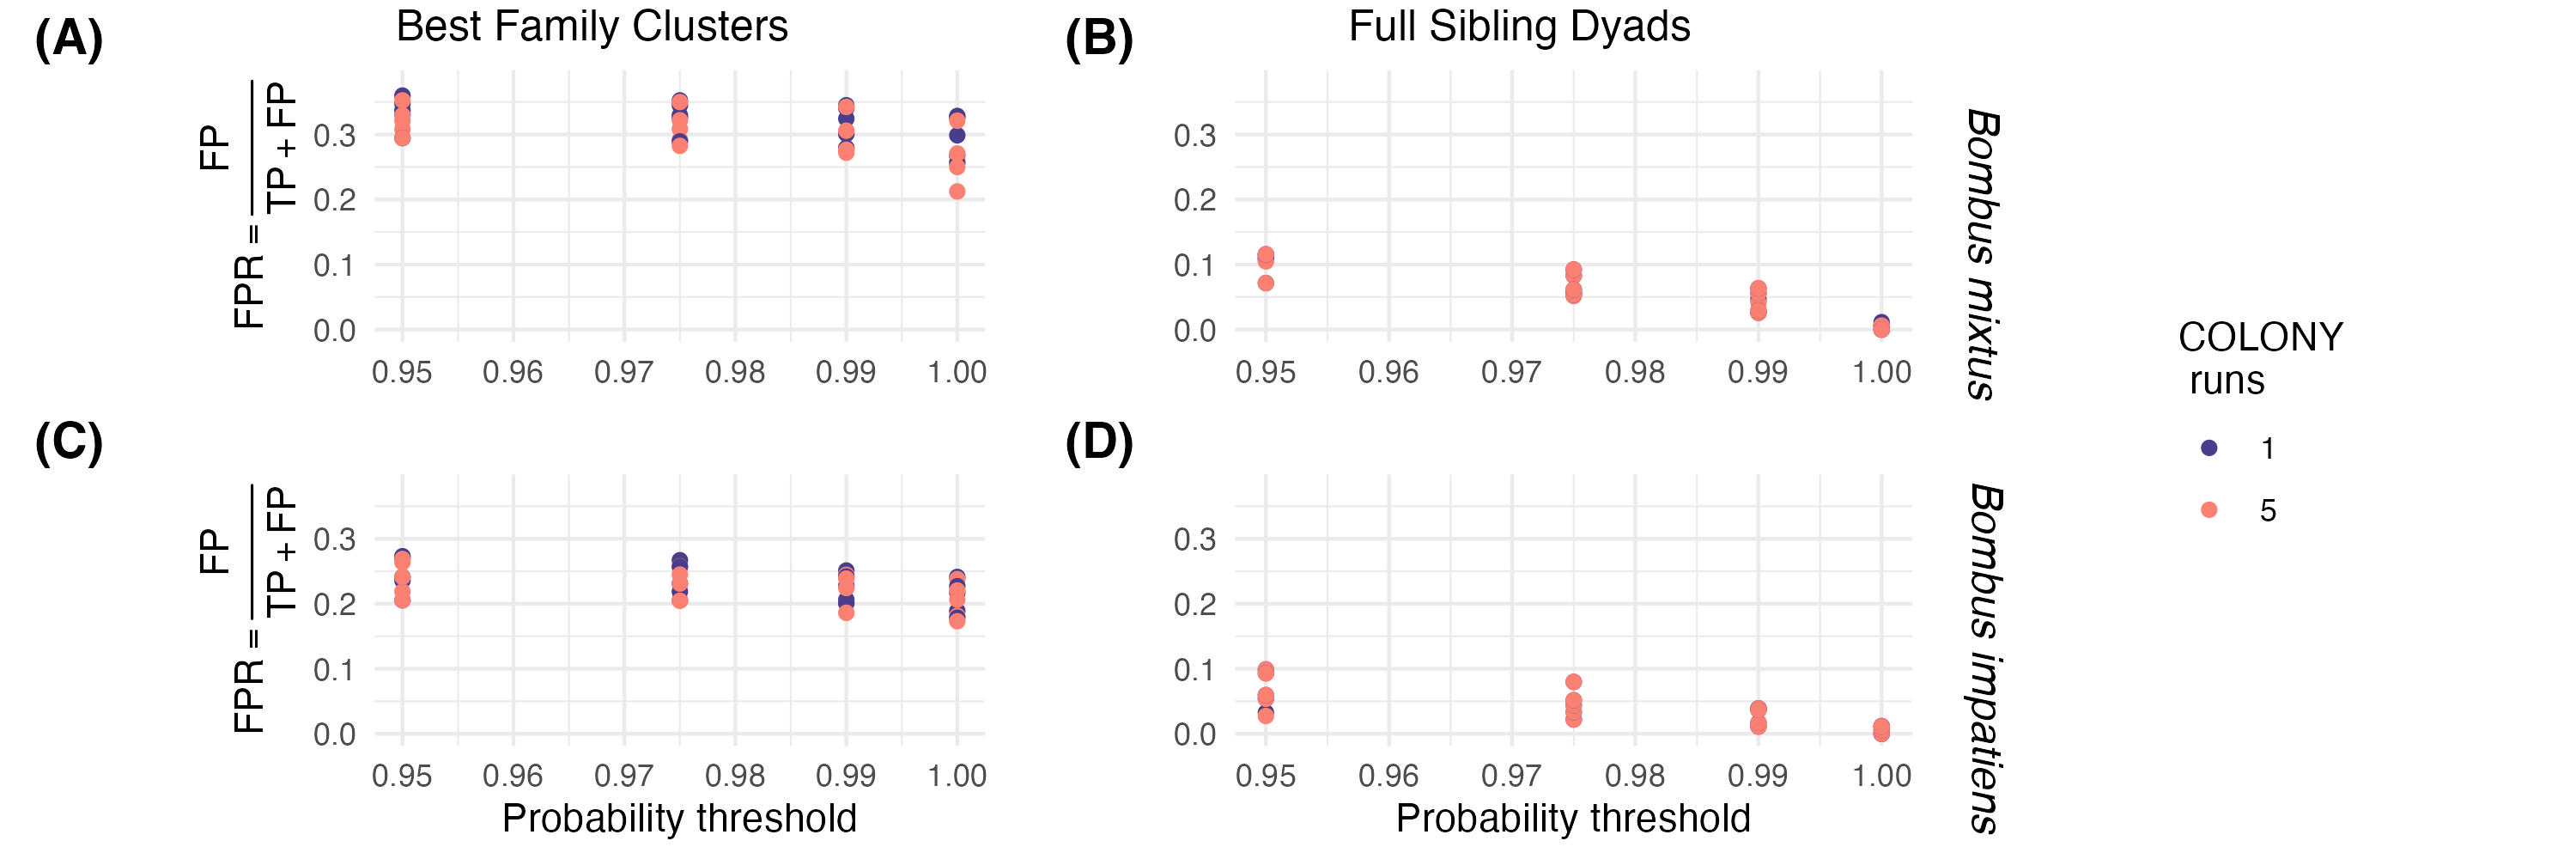
\includegraphics[width=\linewidth]{appendix_figures/fnr_repetition.jpg}
    \caption{False negative rates produced by COLONY 2.0.6.5 when assigning siblingships to simulated data based on \emph{B. mixtus} (A-B) and \emph{B. impatiens} (C-D) allele frequencies and marker numbers. Shown here as a function of the probability threshold used to maintain siblingships. (A, C): False negative rates when siblingships are assigned via the ``family" method (using .BestCluster output), (B, D): False negative rates when siblingships are assigned via the ``dyad" method (using .FullSibDyad output). Color denotes the number of replicated runs of the software used to establish siblingships; a high degree of overlap between the two methods (1 vs 5 runs) suggests that the results of each run are highly stable and that a single run is just as effective as five runs for excluding erroneous siblingships, but that including additional runs of the software does not increase the fall negative rate.}
    \label{fig:fnr_repetition}
\end{figure}


\subsection{Performance of family and dyad methods with and without siblingship size priors}

To fully assess utility of the family method to the dyad method, we need a method for resolving ``non-circular" families. They families arise when some (but not all) individuals in a group are inferred to be full siblings (e.g., A related to B, B related to C, A not related to C). Such cases are rare, and handled internally by COLONY to create \emph{family clusters} that are circular. Because we choose here to refer to dyad pairs rather than family clusters, we are left the task of deciding how to resolve non-circular families. Indeed, resolution of non-circular families could be one process which leads to a higher false positive rate under the family method.

We explored several heuristics for resolving non-circular families. We started by exploring the structure of non-circular families in our simulated datasets, to determine whether non-circularity is more frequently the result of false positives (e.g., a third individual being erroneously added to a sibling pair) or false negatives (e.g., failure to detect a sibling relationship between any pair of siblings in a triad).

To do this, we identified non-circular families from all five simulations, using a threshold of $P = 0.995$ for inclusion of pairwise relationships. When then classified each missing link as either a false negative (a true siblingship that was not inferred by our method) or a true negative (a false siblingship that was correctly excluded, meaning that at least one of the other siblingships in the non-circular family was a false positive). Fig \ref{fig:noncircularity} shows the distribution of false negatives and true negatives in both \emph{B. mixtus} and \emph{B. impatiens}.

\begin{figure}[H]
    \centering
    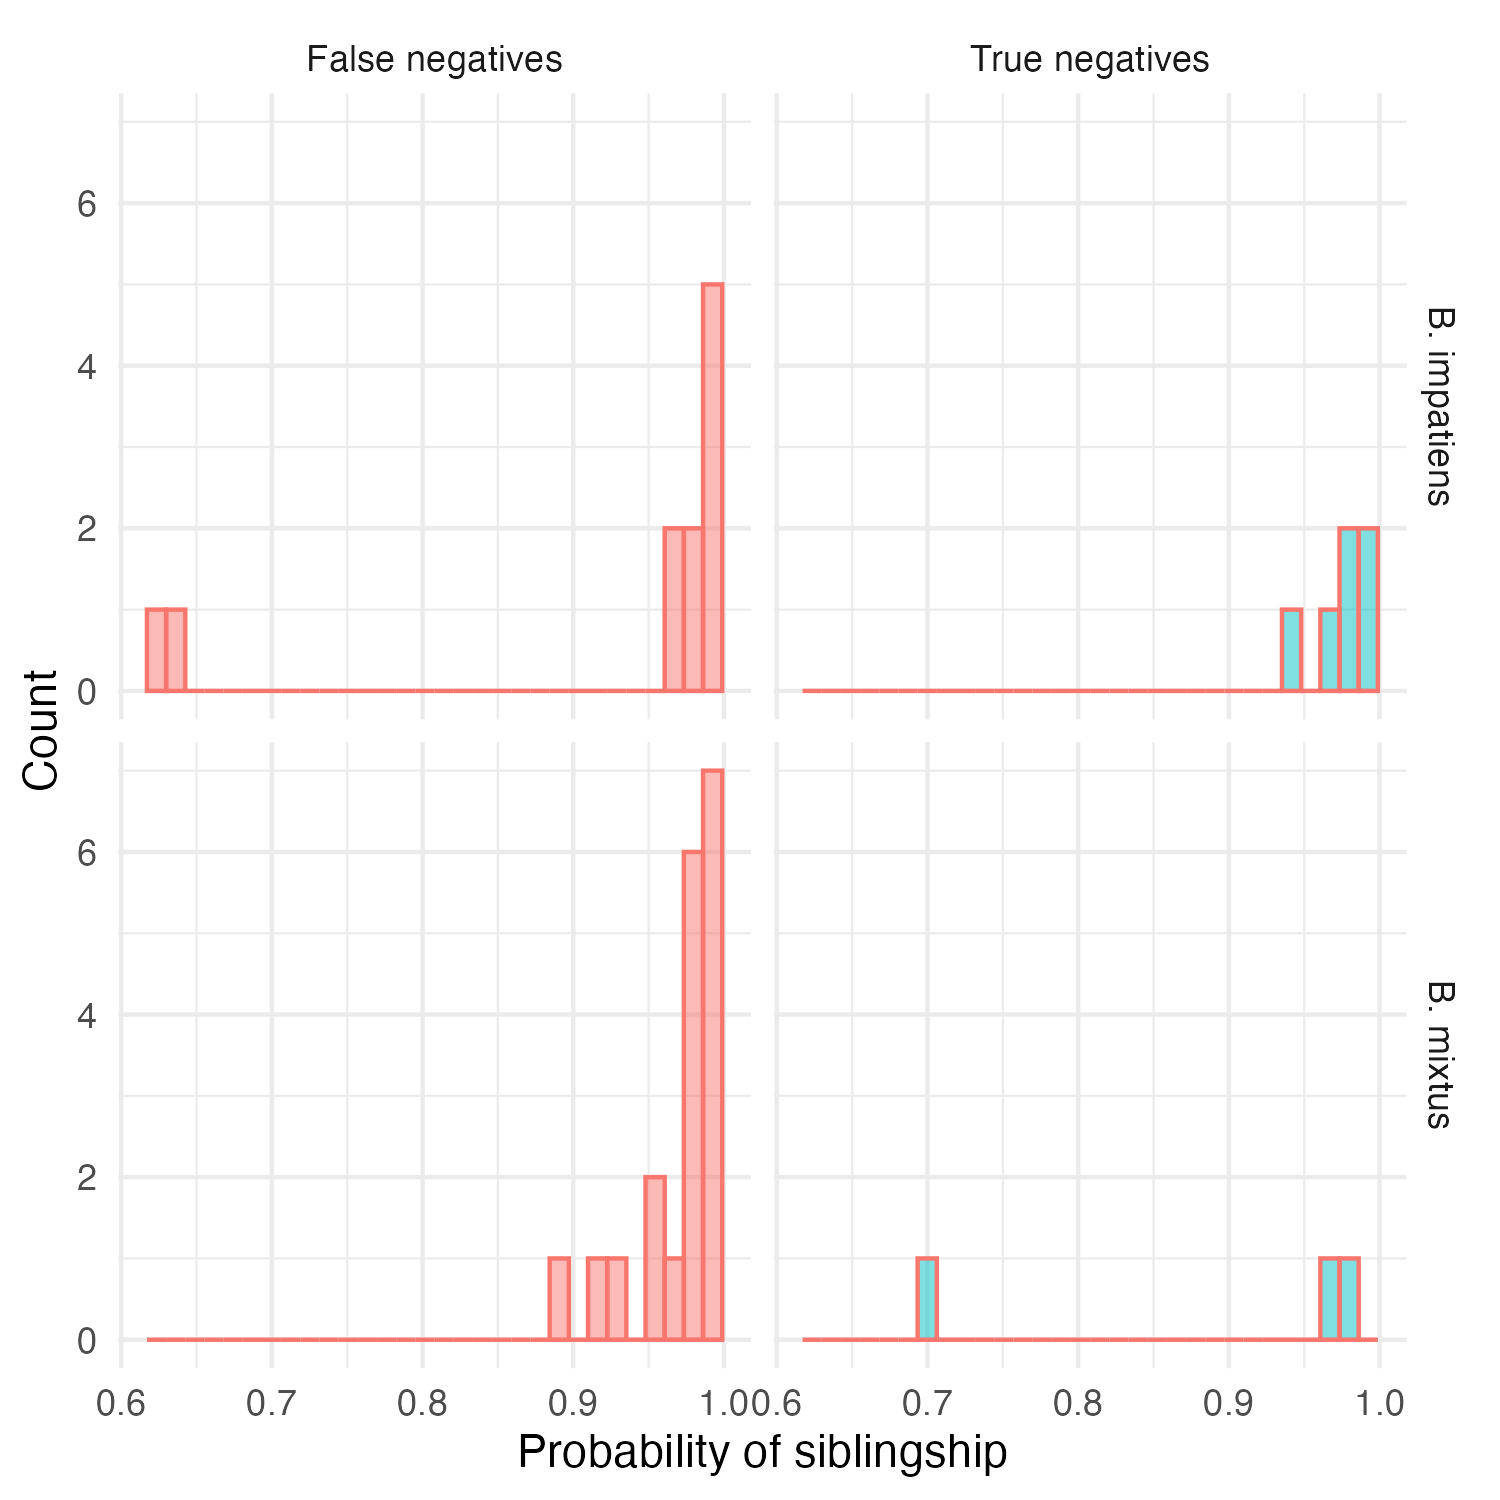
\includegraphics[width=\linewidth]{appendix_figures/noncircularity.jpg}
    \caption{Frequency of false negative and true negative ``missing links" in non-circular siblingships. The x-axis shows the probability assigned to each missing link by the COLONY full sib dyad method (maximum = 0.994, probability threshold for initial acceptance of sibling pairs = 0.995).}
    \label{fig:noncircularity}
\end{figure}

While there does not appear to be a convenient threshold at which we are able to exclude all true negatives while maintaining all false positives, it is comforting that the majority of missed links appear to be false negatives, meaning that we can select a lower probability threshold (e.g., $P = 0.95$) at which to accept these relationships and circularize families without introducing a large number of false positives.

After this step, we are left with a small number of remaining non-circular families (e.g., missing links rejected even at a lower probability threshold). These families are resolved by maintaining the largest ``clique" (e.g., group in which all siblings are connected) or by randomly selecting one complete clique, if they are of equal size.

When comparing the family method to the dyad method for siblingship assignment, we found that results were strongly dependent on whether a siblingship size prior was used. The siblingship prior allows researchers to set a prior on the harmonic mean family size, based on their previous understanding of the expected family sizes in their dataset or similar datasets. Based on our preliminary analyses, about 70-80\% of individuals in our true dataset originated from ``singleton" colonies (no siblings in the dataset), so we set our siblingship priors to 1 individual per family.

For this analysis, we simulated datasets of N = 2000 individuals and subsampled 20\%, 40\%, 60\%, 80\%, or 100\% of individuals to test the use of siblingship priors across datasets of multiple sizes. Our probability threshold was $P = 0.995$. 

When not utilizing a prior, we found that the family method was much less reliable than the dyad method for excluding erroneous siblingships (Fig \ref{sibprior_families}); false negative rates were similar for both strategies. For the family method, 10-60\% of all inferred pairwise relationships were false positives when not using a size prior. False positive rates were consistently $\le 0.2$ when a prior was used (Fig \ref{fig:sibprior_families}). The dyad method, in contrast, resulted in $\le 12\%$ false positives for all conditions tested, and was typically $\le 5\%$ (Fig \ref{fig:sibprior_dyads}). Interestingly, we found that when we assigned siblingships based on the dyads method, the use of a siblingship size prior has little effect on the false positive or false negative rates for \emph{B. mixtus}, but caused a marginal increase in false positives and a marginal decrease in false negatives for \emph{B. impatiens} (Fig \ref{fig:sibprior_dyads}). 

\begin{figure}[H]
    \centering
    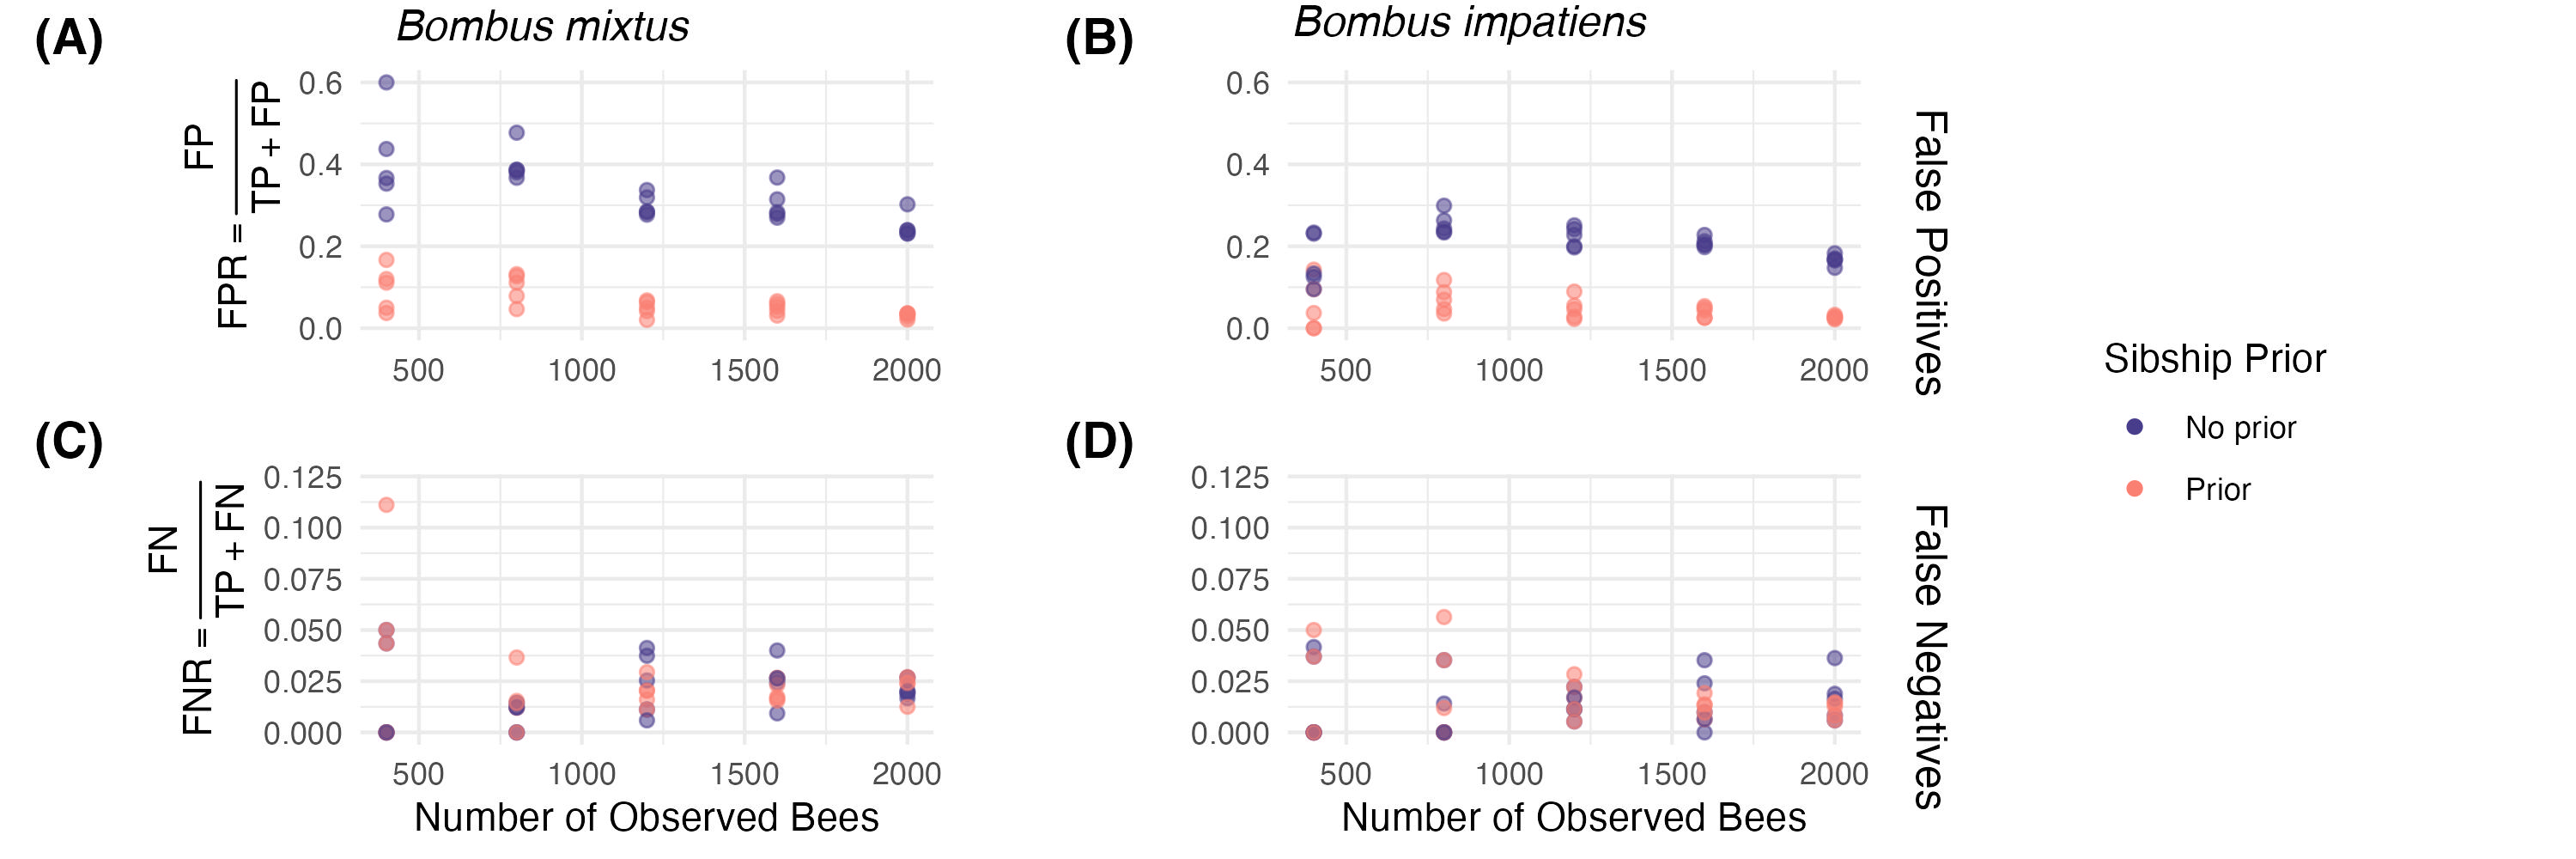
\includegraphics[width=\linewidth]{appendix_figures/sibprior_families.jpg}
    \caption{False positive (A-B) and false negative (C-D) rates of siblingship assignment in \emph{B. mixtus} (A, C) and \emph{B. impatiens} (B, D) using the family assignment method. Dark purple denotes family assignments without the use of a prior on siblingship size, pink denotes family assignments \emph{with} the use of a prior on siblingship size (harmonic mean of siblingship sizes = 1).}
    \label{fig:sibprior_families}
\end{figure}

\begin{figure}[H]
    \centering
    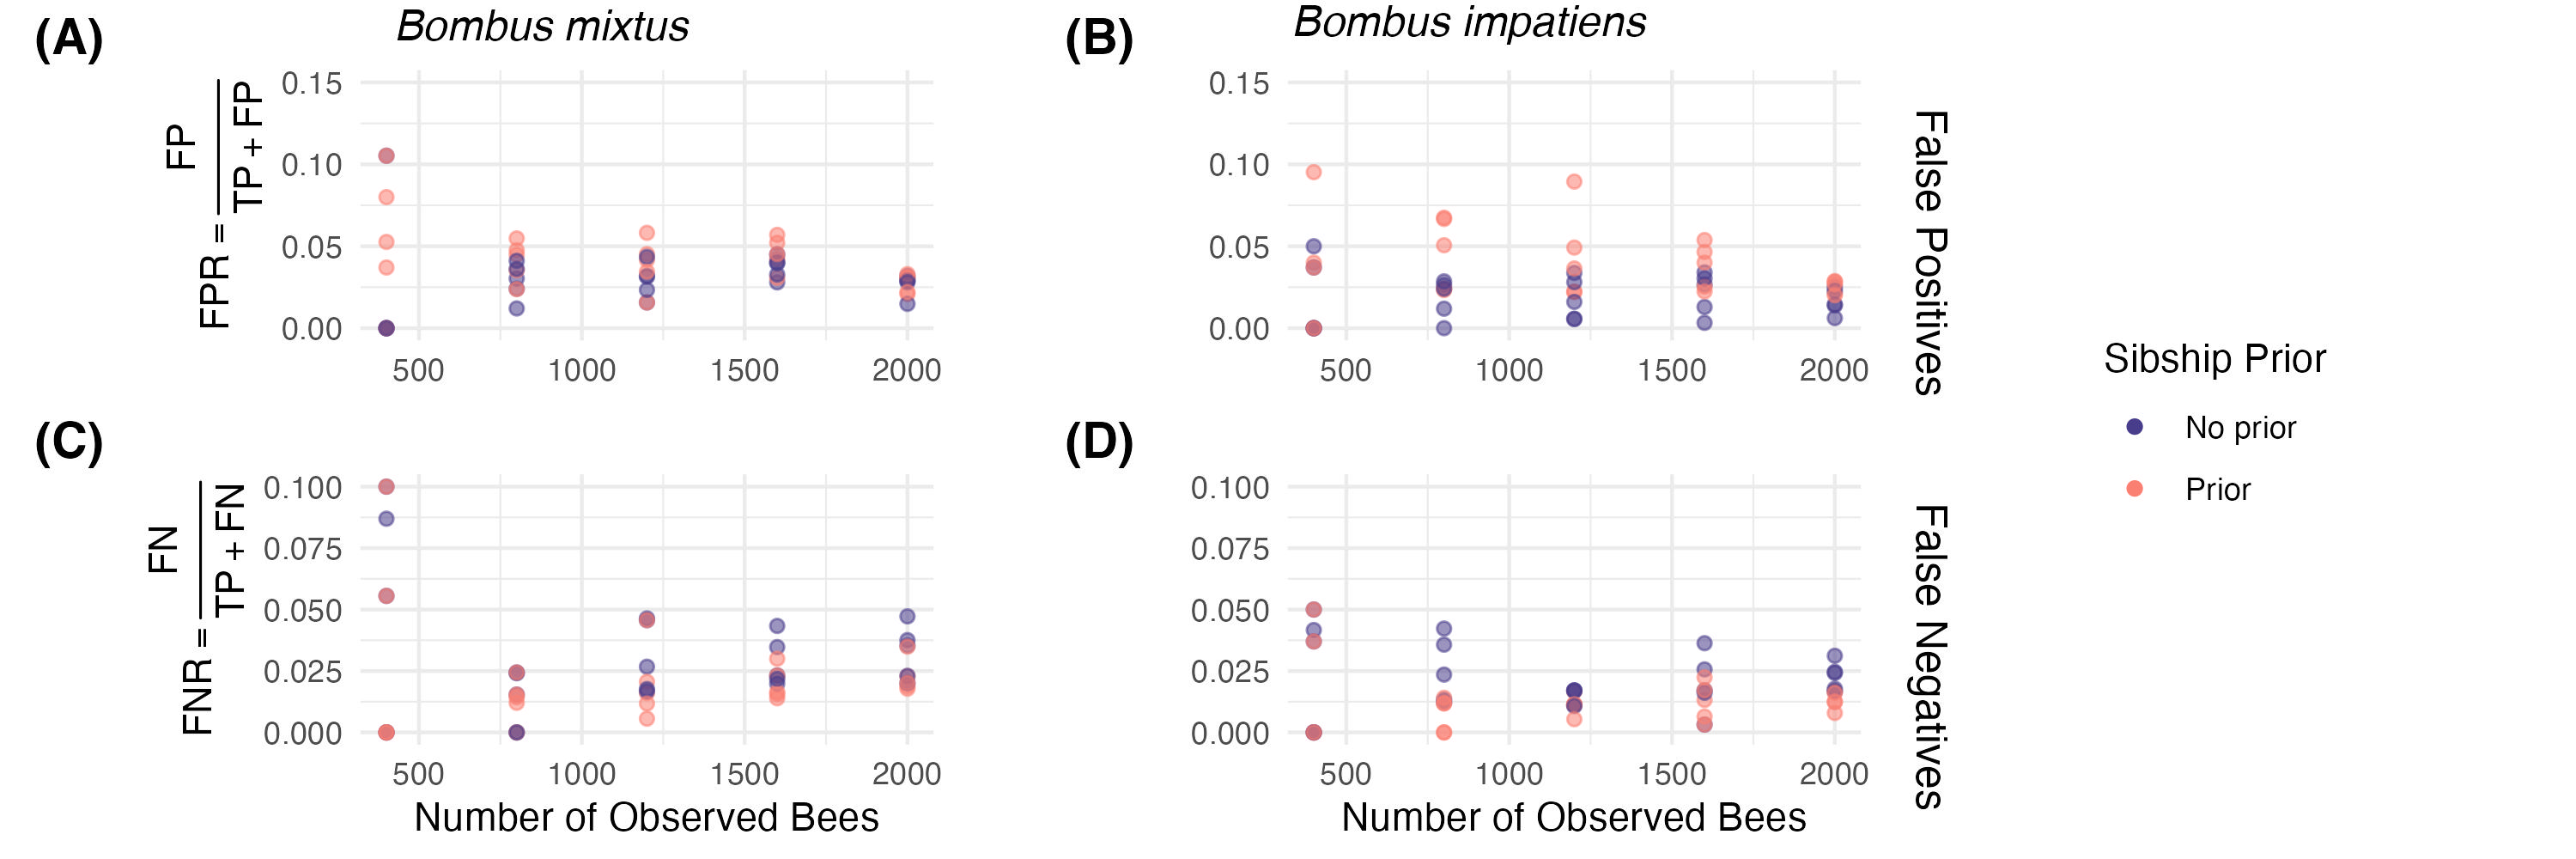
\includegraphics[width=\linewidth]{appendix_figures/sibprior_dyads.jpg}
    \caption{False positive (A-B) and false negative (C-D) rates of siblingship assignment in \emph{B. mixtus} (A, C) and \emph{B. impatiens} (B, D) using the dyad assignment method. Dark purple denotes family assignments without the use of a prior on siblingship size, pink denotes family assignments \emph{with} the use of a prior on siblingship size (harmonic mean of siblingship sizes = 1).}
    \label{fig:sibprior_dyads}
\end{figure}


We did not test for statistical significance, but given the qualitative results we decided to utilize the dyad method with a probability threshold of $P = 0.995$ and no siblingship size prior for our final analysis of real data. 


\subsection{Assessing the use of cross-site sibling exclusion for reducing false positive rates}

We next systematically evaluated the use of a sibling exclusion criteria to determine whether this software specifications improves siblingship inference accuracy. 

Previous studies on \emph{Bombus} have varied in their approaches to the scale at which possible siblingships are evaluated, with some studies performing separate runs of the software for populations sampled at different sites/regions \parencite{jhaResourceDiversityLandscapelevel2013} while others group populations at larger scales, permitting the discovery of long distance foraging or dispersal events between sites \parencite{lepaisEstimationBumblebeeQueen2010, molaWildfireRevealsTransient2020, raoBumbleBeeHymenoptera2012}. While identifying the maximum foraging or dispersal range for different species or landscape contexts is an important goal, we consider two challenges to this method, related to (i) the improbability of capturing individuals engaged in such long distance events, and (ii) the statistical challenges introduced by a very high number of pairwise comparisons between individuals at different sites. For a more thorough discussion of the first point, we direct the reader to \textcite{lepaisEstimationBumblebeeQueen2010a}. Ultimately, we posit that the rate at which long distance foraging events should be captured in the dataset is much lower than both the false positive and false negative rates of the COLONY software, due to the quadratically increasing search area over which foragers will be dispersed as distance from their nest increases (see discussion in \textcite{osborneBumblebeeFlightDistances2008}). Furthermore, given the large sample sizes of our populations, and the fact that the majority of pairwise comparisons (without exclusion) will occur between individuals at different sites, we hypothesized that allowing for siblingship assignments between all individuals would result in a high percentage of false positive relationships that would severely bias estimates of colony locations and foraging behaviour.

To test this hypothesis, and to determine whether total sample size had an effect on the utility of excluding cross-site siblingships, we simulated five datasets of n = 2000 individuals, and subsetted each data set to contain 20, 40, 60, 80, or 100\% of the initial samples. These data were simulated to reflect trapping grids which were arranged in a 3 x 2 grid with traps in adjacent grids at least 6km apart (Fig \ref{fig:simulations} A-B). The minimum distance between adjacent trapping grids in our real data was 5km (also separated by a large river, expected to limit dispersal), and all other sites were at least 7km apart. The mean foraging distance of colonies in our simulation was set to 1km (99\% of all visitations within 3.32km). This would allow for colonies located midway between trapping grids to sampled at two sites, while reflecting the fact that the majority of bumblebee foraging is thought to occur within a few kilometers of the nest. We therefore believe that the simulated data would represent a relatively optimistic view of the number of cross-site siblingships which could be present in the real data.

We created siblingship exclusion tables for COLONY by excluding (for each individual) all potential siblingships with individuals captured at different trapping grids (sites). We ran COLONY on each dataset with and without incorporation of the siblingship exclusion table. Further software specifications for these runs can be found in Table \ref{tab:softwarespecs}. We used the dyad method and an exclusion threshold of $P = 0.995$ as described in the previous section.

We found that for both species (\emph{B. mixtus} and \emph{B. impatiens}) and for all tested sample sizes (n = 400-2000 individuals), cross-site sibling exclusion resulted in a lower false positive rate (Fig \ref{fig:excl_size} A-B). The variation in false positive rates between independent simulations decreased with increasing sample size. When using cross-site exclusion, mean false positive rates were fairly consistent across sample sizes, but without cross-site exclusion, the mean false positive rate tended to decrease with increasing sample size.

False negative rates were similar for both methods, indicating that cross-site exclusion did not cause us to lose a high proportion of real cross-site siblingships (Fig \ref{fig:excl_size} C-D). Indeed, manual inspection of datasets revealed that cross-site sampling was extremely rare or non-existent, given our parameterization and sample size.

Based on these results, we elected to incorporate a between-site sibling exclusion criteria (e.g., only ``look" for siblingships between individuals captured on the same trapping grid) in all further analyses. This includes the section above (e.g., Fig \ref{fig:sibpriordyads}, \ref{fig:sibprior_families}, \ref{fig:fpr_repetition}, \ref{fig:fnr_repetition}).

\begin{figure}[H]
    \centering
    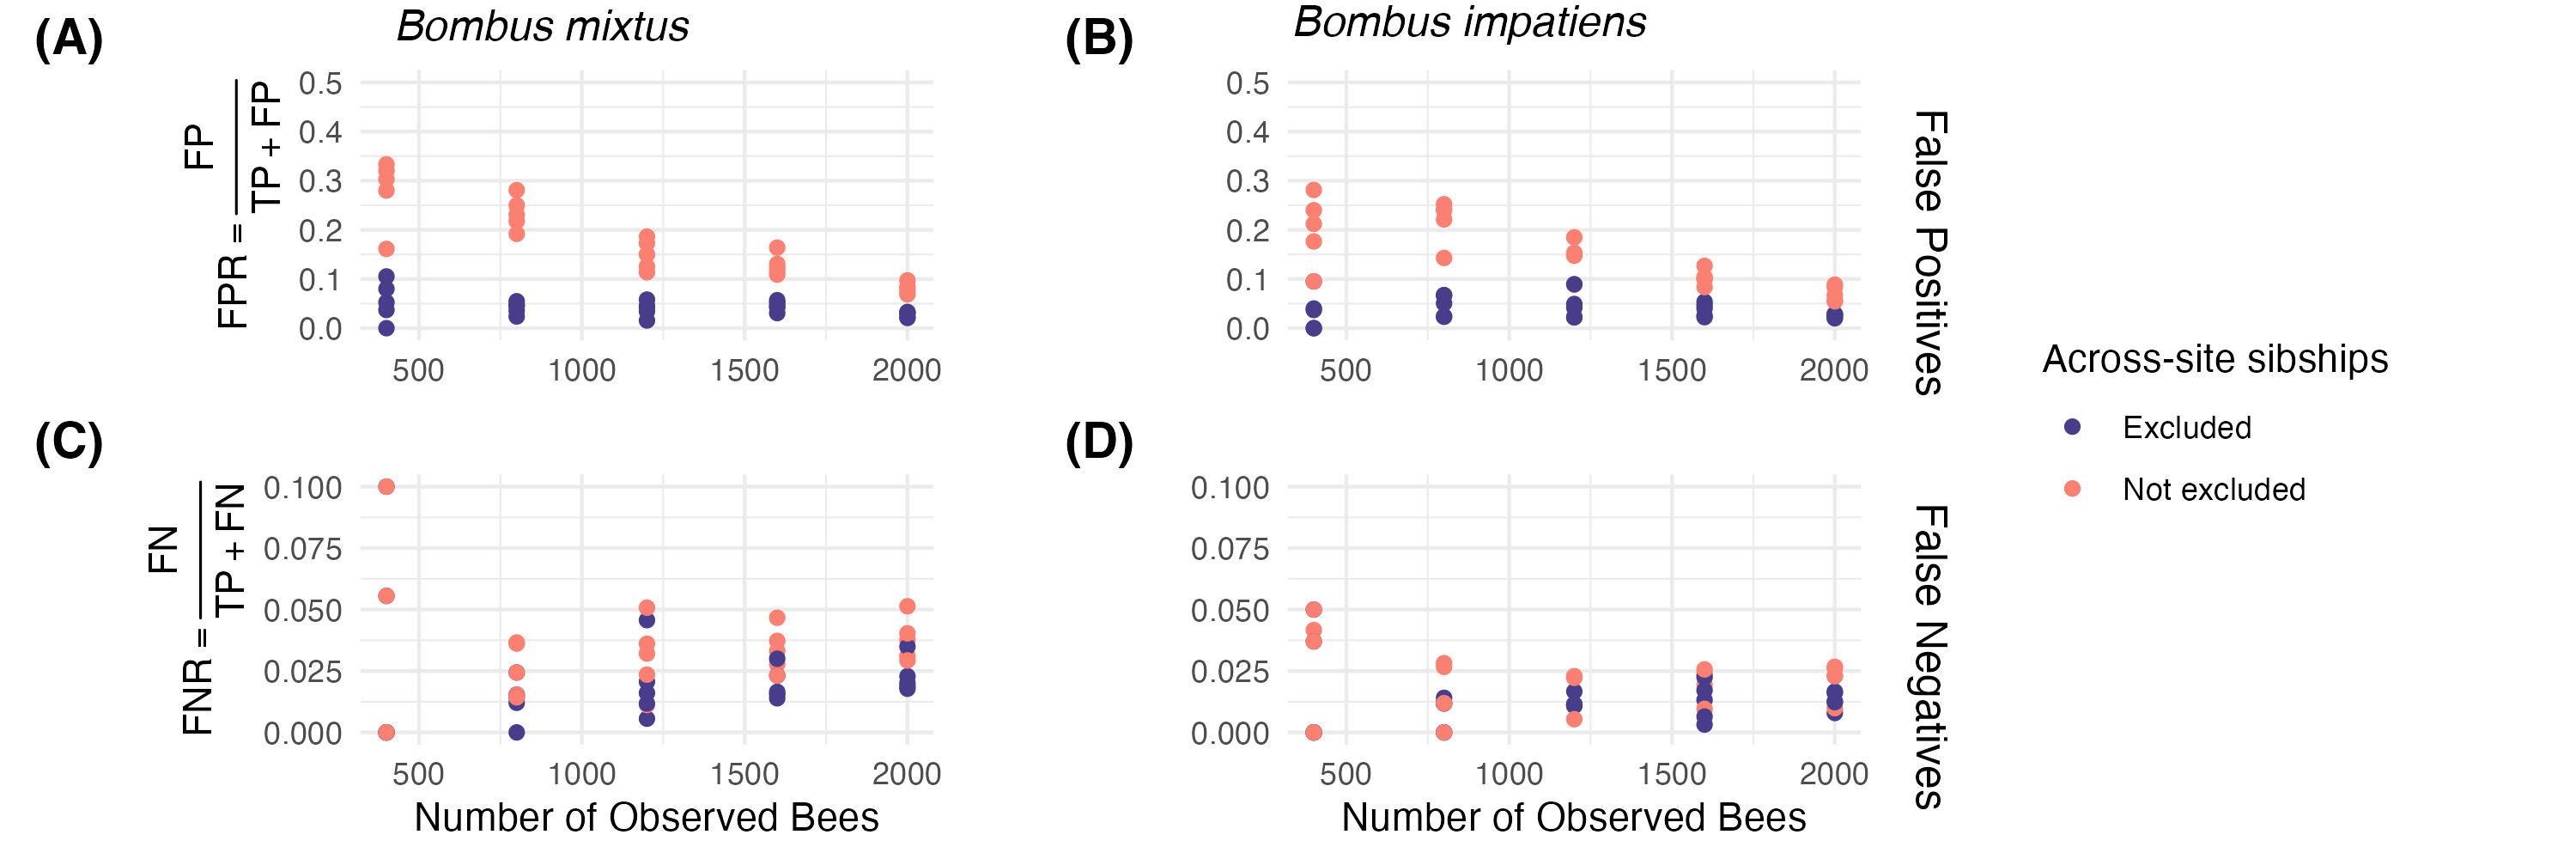
\includegraphics[width=\linewidth]{appendix_figures/excl_size.jpg}
    \caption{Comparison of across-site siblingship exclusion (dark purple) or no exclusion (pink) for minimizing false positive (A-B) and false negative (C-D) rates for \emph{B. mixtus} (A,C) and \emph{B. impatiens} (B,D). Colony assignments were made using the dyad method, with probability threshold = 0.995.}
    \label{fig:excl_size}
\end{figure}


\subsection{Evaluating the effects of multiple paternity on siblingship inference}
% INSERT RESULTS FROM MULTIPLE PATERNITY ANALYSES

\begin{table}[H]
\centering
\caption{Description of software settings (COLONY 2.0.6.5 \parencite{jonesCOLONYProgramParentage2010}) for simulations.}
\label{tab:softwarespecs}
\footnotesize
\begin{tabular}{ p{2cm}  p{3.5cm} p{2cm} p{2.5cm} p{2cm} p{1.5cm}}
\hline
\textbf{Simulation}& \textbf{Comparison}&\textbf{Sample Size}& \textbf{Sibship Size Prior}& \textbf{Cross-site Exclusion}& \textbf{Runs}\\
\hline
\textbf{section 2.2} & Number of COLONY runs& 1200 & yes& yes& 1-5\\
\hline
\textbf{section 2.2} & Probability threshold& 1200 & yes & yes & 1-5\\
\hline
\textbf{section 2.3} & Siblingship size prior & 400-2000 & yes/no & yes/no& 1\\
\hline
\textbf{section 2.2-2.4} & Families vs dyads & 400-2000 & yes/no & yes& 1-5\\
\hline
\textbf{section 2.4} & Cross-site exclusion & 400-2000 & yes/no & yes/no& 1\\
\hline
\textbf{section 2.5} & Mating system& 1000 & no & no& 1\\
   \hline  
\textbf{section 2.5} & Mating system (augmented data)& 1000 & yes & no& 1 \\
   \hline  
\end{tabular}
\end{table}



\end{document}